\documentclass[UTF8]{ctexart}
\usepackage{geometry}
\usepackage{graphicx}
\usepackage{ulem}
\usepackage{blindtext}
\usepackage{index}
\usepackage{fancyhdr}
\usepackage{subfigure} 
\usepackage{wrapfig}
\usepackage[colorlinks,linkcolor=black]{hyperref}
\geometry{a4paper, centering, left = 4cm, right = 4cm}
\newenvironment{intro}{\begin{quote}\kaishu}{\end{quote}}

\usepackage{fancyhdr}                                
\usepackage{lastpage}                                           
\usepackage{layout}                                 
\ctexset{
    section = {
        format = \raggedright\Large\bfseries,
    }
}


%\pagestyle{empty}                  %不设置页眉页脚            
\footskip = 10pt                                                
\pagestyle{fancy}                   % 设置页眉                                                
% \lhead{}                    
\chead{毛泽东思想和中国特色社会主义理论体系概论实践报告}                                                
\rhead{ \thepage\ }                                                
% \cfoot{第 \thepage\ 页\quad 共 \pageref{LastPage} 页}   
\cfoot{}                                              
% \rfoot{页脚左}%                                                       
% \lfoot{页脚右}                                                        
\renewcommand{\headrulewidth}{1pt} %页眉线宽,设为0可以去页眉线
% \setlength{\skip\footins}{2cm}   %脚注与正文的距离           
% \renewcommand{\footnotesize}{0pt}     %设置脚注字体大小           
% \renewcommand{\footrulewidth}{0pt} %脚注线的宽度           
\setlength{\parskip}{0.5em} 
\begin{document}
\fancypagestyle{plain}
\fancyhf{}
\begin{titlepage}
    \begin{figure}[h]
        \centering
        \includegraphics[width=9cm]{imgs/logo.jpg}
    \end{figure}
    \vskip 35mm
    \begin{center}
        \normalfont
        {\Large\bfseries 毛泽东思想和中国特色社会主义理论体系概论实践报告}
        
        \vskip 10mm
        \normalfont{\Huge\bfseries 瞻前与顾后}

        \vskip 30mm
        {\Large\itshape 丁优龙}{\Large 2019151088}

        % \medskip
        % {\Large\itshape 费楚雯}{\Large 2019191139}
        
        % \medskip
        % {\Large\itshape 董芸豪}{\Large 2019284073}
        
        % \medskip
        % {\Large\itshape 霍晓雨}{\Large 2019151092}
    \end{center}
    \vspace{\stretch{0}}
\end{titlepage}
\clearpage
\section*{\Large 实践主题}
探访文化之根、促进中外交流\raisebox{0.5mm}{------}中外友人南头古城之旅
\section*{\Large 实践目的}
位于深圳中心区域的南头古城始于晋代,直至新中国建国初期,历代都是深港地区的政治、军事和经济中心,为加深对深圳文化历史的了解,促进国际文化交流共通,粤桂社区党委联合深圳大学国际交流学院各外籍学生,以及其他学院的中国志愿者,组织了一次别开生面的文化交流活动,共同前往深圳文化之根南头古城。
\section*{\Large 实践时间}
2020年11月6日下午2:00---5:00
\section*{\Large 实践地点}
深圳市南山区南头古城
\section*{\Large 实践形式}
在南头古城导游的带领下,我作为志愿者随同外国友人游览南头古城风貌并承担同步翻译的任务。游览环节包括参观1820数字展馆,同源馆,品尝南头古城特色美食,进行友好互动及交流。本次探访交流之旅有来自中国、巴基斯坦、美国、日本、韩国、越南、柬埔寨、俄罗斯、印度共9个国家的学生,各位学生互相沟通,互相碰撞。
\clearpage
\section*{\Large 正文}
\begin{figure}[h]
    \centering
    \includegraphics[width=8cm]{imgs/overlook.jpg}
    \begin{center}
        \Large\bfseries 瞻前与顾后
    \end{center}
\end{figure}

一整天都在架构社会实践报告,直到傍晚,我才饥肠辘辘地跳入对面的桂庙,准备胡乱觅些甜食。12月的鹏城终于入冬,从寒风暮色里躲进暖色调的小厅,还没来得及喘口气,忽见展示台上放着糖水,我不禁莞尔一笑,好像我到广东来的记忆里,还没怎么品尝过什么样子粤菜的印象,都是上课、学习、实验室、教室$\cdots \cdots$不过,我当然记得,记得上个月在南头古城所知所感的所有味道。

\begin{center}
    (一)
\end{center}

南头古城之旅其实只有半天,在我刚踏上大巴车的一刻,感觉自己仿佛身在异国他乡:周围坐满了来自世界各地的外国友人们,有的在低头看报,有的在轻声交流,在想要打个招呼又怕打扰到他们的犹豫中,我走到了后排的一个空位坐下。"Hello, everyone! Welcome to \dots",大巴缓缓驱动,我拿起话筒,开始了我的工作任务。

\begin{center}
    (二)
\end{center}

对于南头古城的第一印象,在于那座挂着“岭南重镇”的古城墙(见图1),上一秒还坐着大巴在高楼林立的都市中穿梭,下一秒的画面就切换到了古时岭南重镇的南大门,时空的巨大跳跃不免让人有些恍惚。导游人员开始用中文介绍深圳发展历史上的十三个转折点,时间线始于千年前的东晋,贯穿到上世纪80年代改革开放。


历史的重要意义,唐皇早已指出:如明镜般可察人情、可知兴衰,这是固然是一个统治者的阅读需要,然而,今天的读者阅读历史往往是满足于简单的好奇、通俗的娱乐、浅显的认知,了解渠道不外乎大众读物、影视改编、百家讲坛。其实,历史的价值对于今人更是自我认识的启蒙,历史中真实的内心、变形的人形、丰富的人性才是研究的对象。倘若将太宗的一面明镜改变形态,历史的视角也将产生奇巧而深刻的变化。

有人认为历史是展望未来的望远镜,我却并不苟同,未来变化无穷、科技日新月益,而历史是停留在当时的智慧,不可能预示和解决未来的一切难题。但历史可以是帮助未来人们规避风险的反光镜,历史的教训、成功的经验,的确对于现实弥足珍贵。不过,“以史为镜”只可远照未来或反视过去,就低估了历史的价值,也小看了镜子的功能。

\begin{figure}[htbp]
    \centering
    \subfigure[图1:城门前的合影,笔者(左一)]{
    \begin{minipage}[t]{0.5\linewidth}
    \centering
    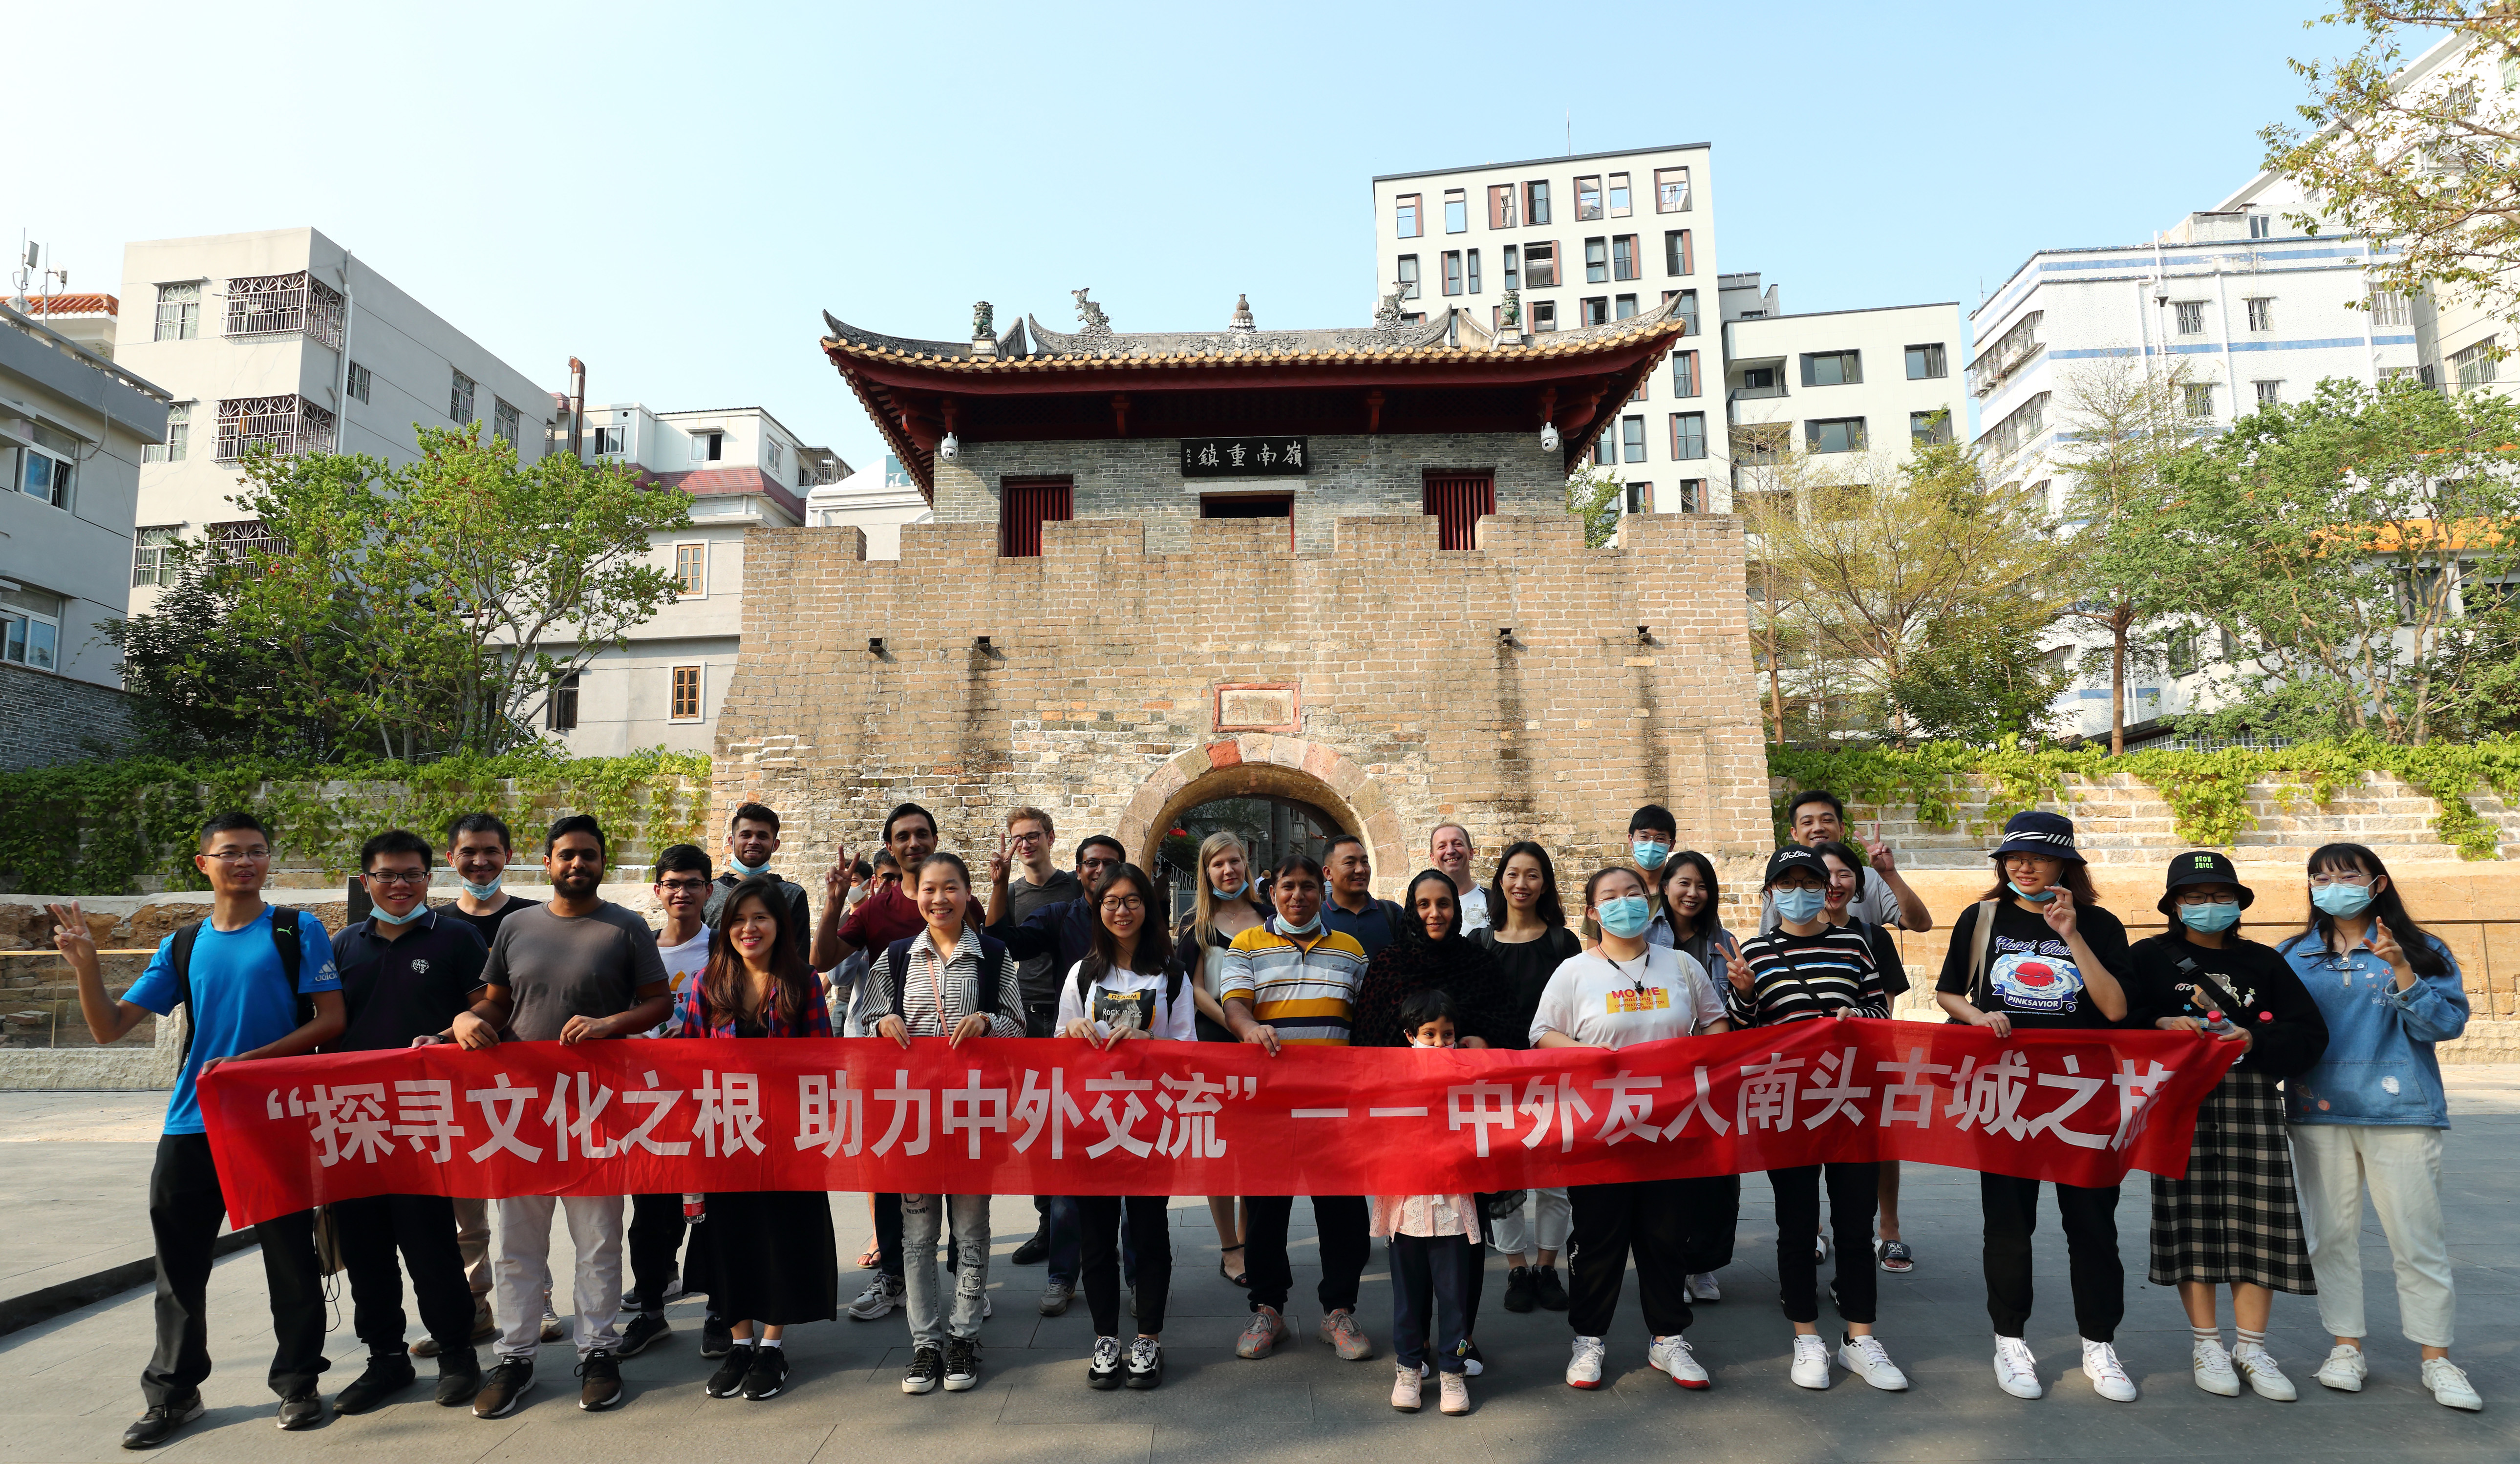
\includegraphics[width=5.5cm]{imgs/gate.JPG}
    % \caption{figffff1}
    \end{minipage}%
    }%
    \subfigure[图2:路过襟江酒家(右)]{
    \begin{minipage}[t]{0.5\linewidth}
    \centering
    \includegraphics[width=5.5cm]{imgs/wine.JPG}
    % \caption{fig2}
    \end{minipage}%
}
\end{figure}
\begin{center}
    (三)
\end{center}

\begingroup
\setlength{\intextsep}{0pt}
\setlength{\columnsep}{15pt}

\begin{wrapfigure}{r}{0.45\textwidth}
  \centering
  \includegraphics[width=5.5cm]{imgs/reform.jpg}
\end{wrapfigure}
资料显示,去年3月,南头古城作为“深圳十大特色街区之一”进入项目提升改造阶段,改造后的南头古城主要结合文创精品零售、传统特色餐饮等,打造成融合传统文化和现代创意的特色文化街区(见右图)。此行的游览中,我们也正好路过了已经改造完成的襟江酒家(见图2)。新闻报道称,今年的十一黄金周中,南头古城展现出火爆的人气。看来,改造后的南头古城俨然成为了文化旅游目的地。其实,南头古城并非个例。早在2017年时,故宫就深度挖掘明清皇家文化元素与丰富文物资源,大力发展文创等衍生品产业,一年文创产品即创造15亿的产值,且大多反哺故宫文物修复和文物保护。由此可见,越来越多的优秀传统文化纷纷走出“故纸堆”,以时尚有趣形象“飞入寻常百姓家”。

\begin{wrapfigure}{l}{0.45\textwidth}
    \centering
    \includegraphics[width=5.5cm]{imgs/digital.jpeg}
  \end{wrapfigure}

分析两者的成功之处,不难发现,它们都是激活传统文化的大众需求,结合最新科技,使历史的温度仍能燃烧出全新的热力,散发出新时代的光芒。我想,这些也恰给当今传统文化的继承与发展提供了一个全新的思路。

\endgroup
\begin{center}
    (四)
\end{center}

在导游人员介绍地面铺砌的石头时,我全程陪同的一位德国白人小哥用英文问我:“她(导游)在说的是石头吗,石头用中文要怎么说”,当我告诉他答案后,我们同时露出了惊讶的表情,原来,“石头”和“stone”的发音是如此相近。这是一个很有趣的巧合,异域文化间类似的巧合与共通之处数不胜数。越是民族的,越是世界的,周恩来总理曾巧妙地将《梁山伯与祝英台》改为“中国的《罗密欧与朱丽叶》”,爱情悲剧的基调,一下子拉近了与西方观众的距离。然而,文化的跨区域流动并非一帆风顺,许多偏见与误解,正是源于对不同文化的片面认知。前些年,美国哥伦比亚大学校园内,一些中国留学生的宿舍门牌上因为有中文拼音名字,而被有意撕毁。在当今世界格局下,文化作为综合国力的一部分,其输出问题也越来越受到重视。想到去年年底,话题“李子柒到底是不是文化输出”上了微博的热搜榜,无论如何不可否认的是,李子柒的视频让外国网友对中国文化产生了向往和喜爱之情,也让中国文化走向了世界,可见诸如此类的文化输出是成功的,同时也让也让我们意识到:在当今的互联网语境下,文化输出并不是一件多么严肃的事,也并不只是官方的事,文化输出的平民化,正成为一种新的趋势。

\begin{center}
    (五)
\end{center}

关于历史的思考,文化的思考,启发还是很多很多。但愿今后能有时间一一回顾。最后的句子只是随想随感。

无论是半天,还是半年,无论地球有多么小,时间有多么大,时间的流动,空间的跳跃,总是让我们感到恍惚,想必大巴车上又会有新的伙伴,屹立的城墙还是看淡人间风雨$\cdots \cdots$但谁能看到想法和内心的变化呢,谁能知眼光和心思的不同呢?我终于理解“给我一个支点,我可以撬动地球”的意思了。

我虽然未曾品尝到那碗糖水,但我尝过无比的味道。相信未来可期,美味可施,青山常在,绿水长流。
\end{document}